\documentclass[12pt]{article}
\usepackage{amsthm}
\usepackage{amsmath}
\usepackage{array}
\usepackage{cancel}
\usepackage[thinc]{esdiff}
% \usepackage{gensymb}
\usepackage{geometry}
\usepackage{graphicx}
\usepackage{pgfplots}
\usepackage{siunitx}
\usepackage{wrapfig}
\usepackage{xcolor}

\title{Homework \#10, 4B}
\author{Donald Aingworth IV}
\date{March 26, 2025}

\pgfplotsset{width=8cm,compat=1.9}
\usepgfplotslibrary{external}
% \tikzexternalize

\renewcommand\thesubsection{\alph{subsection}}
\newcommand{\proj}{\text{proj}}
\newtheorem{theorem}{Theorem}

\begin{document}

\DeclareSIUnit{\mile}{mi}
\DeclareSIUnit{\gal}{gal}
\DeclareSIUnit{\foot}{ft}
\DeclareSIUnit{\hour}{h}
\DeclareSIUnit{\rad}{rad}
\DeclareSIUnit{\unit}{u}
\DeclareSIUnit{\dyne}{dyn}

\section{Chapter 21, Problem 71}
In a spherical metal shell of radius $R$, an electron is shot from the center directly toward a tiny hole in the shell, through which it escapes. The shell is negatively charged with a surface charge density (charge per unit area) of $6.90 \times 10^{-13} \unit{\coulomb/\meter^2}$. What is the magnitude of the electron's acceleration when it reaches radial distances (a) r = 0.500R and (b) 2.00R?

\section{Chapter 22, Problem 71}
A charge of $20  \unit{\nano\coulomb}$ is uniformly distributed along a straight rod of length $4.0  \unit{\meter}$ that is bent into a circular arc with a radius of $2.0 \unit{\meter}$. What is the magnitude of the electric field at the center of curvature of the arc?

\section{Chapter 22, Problem 83}
An electric dipole with dipole moment
\[\vec{p} = (3.00\hat{i} + 4.00\hat{j})(1.24 \times 10^{-30} \unit{\coulomb\meter})\]
is in an electric field $\vec{E} = (4000 N/C)\hat{i}$. (a) What is the potential energy of the electric dipole? (b) What is the torque acting on it? (c) If an external agent turns the dipole until its electric dipole
moment is
\[\vec{p} = (-4.00\hat{i} + 3.00\hat{j})(1.24 \times 10^{-30} \unit{\coulomb\meter})\]
how much work is done by the agent?

\section{Chapter 23, Problem 78}
A charge of $6.00 \unit{\pico\coulomb}$ is spread uniformly throughout the volume of a sphere of radius $r = 4.00 \unit{\centi\meter}$. What is the magnitude of the electric field at a radial distance of (a) $6.00 \unit{\centi\meter}$ and (b) $3.00 \unit{\centi\meter}$?

\section{Chapter 23, Problem 81 (Challenge)}
A spherical ball of charged particles has a uniform charge density. In terms of the ball's radius R, at what radial distances (a) inside and (b) outside the ball is the magnitude of the ball's electric field equal to $\frac{1}{4}$ of the maximum magnitude of that field?

\section{Chapter 24, Problem 75}
An electric field of approximately 100 V/m is often observed near the surface of Earth. If this were the field over the entire surface, what would be the electric potential of a point on the surface? (Set V = 0 at infinity.)

\section{Chapter 24, Problem 87}
Three $+0.12 \unit{\coulomb}$ charges form an equilateral triangle $1.7 \unit{\meter}$ on a side. Using energy supplied at the rate of $0.83 \unit{\kilo\watt}$, how many days would be required to move one of the charges to the midpoint of the line joining the other two charges?

\section{Chapter 24, Problem 100}
An alpha particle (which has two protons) is sent directly toward a target nucleus containing 92 protons. The alpha particle has an initial kinetic energy of $0.48 \unit{\pico\joule}$. What is the least center-to-center distance the alpha particle will be from the target nucleus, assuming the nucleus does not move?

\section{Chapter 25, Problem 6+}
You have two flat metal plates, each of area $1.00 \unit{\meter^2}$, with which to construct a parallel-plate capacitor. (a) If the capacitance of the device is to be $1.00 \unit{\farad}$, what must be the separation between the plates? (b) Could this capacitor actually be constructed? (c) If the plates were to double in area, what would the new capacitance be?

\section{Chapter 25, Problem 32+}
A parallel-plate air-filled capacitor having area $40 \unit{\centi\meter^2}$ and plate spacing $1.0 \unit{\milli\meter}$ is charged to a potential difference of $600 \unit{\volt}$. Find (a) the capacitance, (b) the magnitude of the charge on each plate, (c) the stored energy, (d) the electric field between the plates, and (e) the energy density between the plates.\\
Suppose that the spacing were increased from $1.0 \unit{\milli\meter}$ to $5.0 \unit{\milli\meter}$. Find (f) the capacitance, (g) the magnitude of the charge on each plate, (h) the stored energy, (i) the electric field between the plates, and (j) the energy density between the plates.

\section{Chapter 25, Problem 50}
\begin{wrapfigure}{r}{0.25\textwidth}
    \vspace{-30pt}
    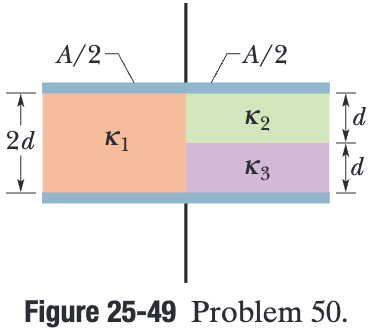
\includegraphics[width=0.25\textwidth]{picture_11.png} 
    % \label{fig:wrapfig}
\end{wrapfigure}
Figure 25-49 shows a parallel-plate capacitor of plate area $A = 10.5 \unit{\centi\meter^2}$ and plate separation $2d = 7.12 \unit{\milli\meter}$. The left half of the gap is filled with material of dielectric constant $\kappa_1 = 21.0$; the top of the right half is filled with material of dielectric constant $\kappa_2 = 42.0$; the bottom of the right half is
filled with material of dielectric constant $\kappa_3 = 58.0$. What is the capacitance?

\section{Chapter 25, Problem 80}
A capacitor is charged until its stored energy is $4.00 \unit{\joule}$. A second capacitor is then connected to it in parallel. (a) If the charge distributes equally, what is the total energy stored in the electric fields? (b) Where did the missing energy go?

\section{Chapter 23, Problem 60}
\textit{The chocolate crumb mystery, Part 1.} Explosions ignited by electrostatic discharges (sparks) constitute a serious danger in facilities handling grain or powder. Such an explosion occurred in chocolate crumb powder at a biscuit factory in the 1970s. Workers usually emptied newly delivered sacks of the powder into a loading bin, from which it was blown through electrically grounded plastic pipes to a silo for storage. Somewhere along this route, two conditions for an explosion were met: (1) The magnitude of an electric field became $3.0 \times 10^6 \unit{\newton/\coulomb}$ or greater, so that electrical breakdown and thus sparking could occur. (2) The energy of a spark was $150 \unit{\milli\joule}$ or greater so that it could ignite the powder explosively. Let us check for the first condition in the powder flow through the plastic pipes.\\
Suppose a stream of negatively charged powder was blown through a cylindrical pipe of radius $R = 5.0 \unit{\centi\meter}$. Assume that the powder and its charge were spread uniformly through the pipe with a volume charge density $\rho$. (a) Using Gauss' law, find an expression for the magnitude of the electric field $\vec{E}$ in the pipe as a function of radial distance $r$ from the pipe center. (b) Does E increase or decrease with increasing $r$? (c) Is $\vec{E}$ directed radially inward or outward? (d) For $\rho = 1.1 \times 10^{-3} \unit{\coulomb/\meter^3}$ (a typical value at the factory), find the maximum E and determine where that maximum field occurs. (e) Could sparking occur, and if so, where? (The story continues with Problem 70 in Chapter 24.)

\section{Chapter 24, Problem 70}
\textit{The chocolate crumb mystery, Part 2.} This story begins with Problem 60 in Chapter 23. (a) From the answer to part (a) of that problem, find an expression for the electric potential as a function of the radial distance r from the center of the pipe. (The electric potential is zero on the grounded pipe wall.) (b) For the typical volume charge density $\rho = -1.1 \times 10^{-3} \unit{\coulomb/\meter^3}$, what is the difference in the electric potential between the pipe's center and its inside wall? (The story continues with Problem 60 in Chapter 25.)

\section{Chapter 24, Problem 60}
\textit{The chocolate crumb mystery.} This story begins with Problem 60 in Chapter 23. As part of the investigation of the biscuit factory explosion, the electric potentials of the workers were measured as they emptied sacks of chocolate crumb powder into the loading bin, stirring up a cloud of the powder around themselves. Each worker had an electric potential of about $7.0 \unit{\kilo\volt}$ relative to the ground, which was taken as zero potential. (a) Assuming that each worker was effectively a capacitor with a typical capacitance of $200 \unit{\pico\farad}$, find the energy stored in that effective capacitor. If a single spark between the worker and any conducting object connected to the ground neutralized the worker, that energy would be transferred to the spark. According to measurements, a spark that could ignite a cloud of chocolate crumb powder, and thus set off an explosion, had to have an energy of at least $150 \unit{\milli\joule}$. (b) Could a spark from a worker have set off an explosion in the cloud of powder in the loading bin?

\end{document}